
\chapter{K-Nearest Neighbor}

Imagine assigning each feature a numeric value, and putting them as coordinates in a feature space. To find which label to give to an example $d$ we can see the k-nearest neighbors. The correct label will be the one that has the majority in k neighbors. 


In cases where features are comparable (each feature has the same units) we will use the simple method of Euclidean Distance: 

\[
D(a,b) = \sqrt{(a_1-b_1)^2+(a_n-b_n)^2}
\]

\section{Decision boundaries}

\begin{definition}[Decision boundaries]
	Decision boundaries are places where the the classification of an example changes.
\end{definition}

These boundaries are a subset of the Voronoi diagram which divides the initial points distribution by equidistant lines. 

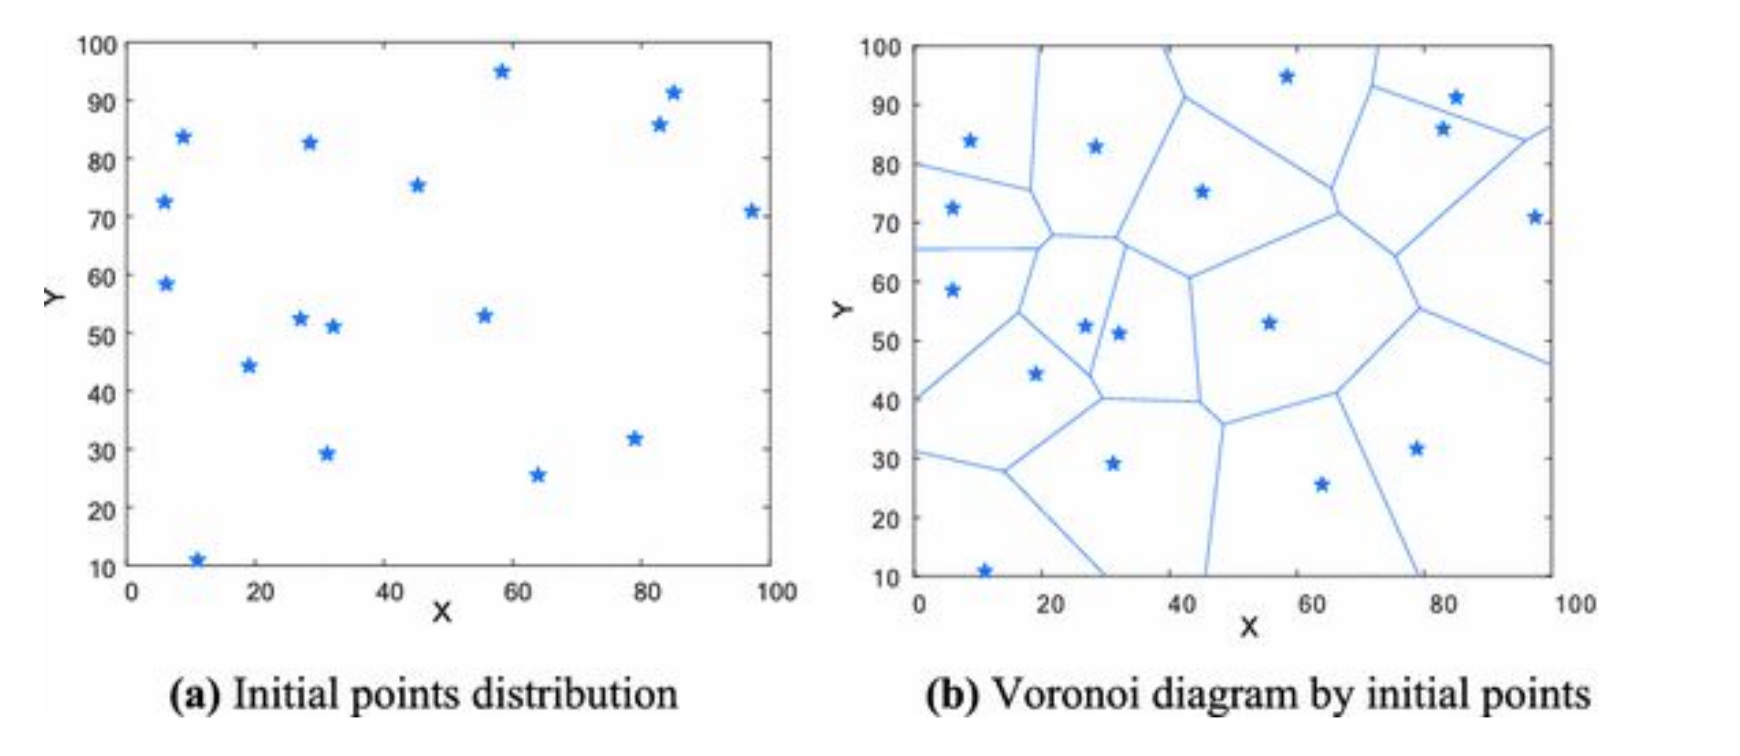
\includegraphics[scale=0.2]{voronoi}

Choosing K will have an effect on underfitting and overfitting.

\begin{definition}[Underfitting]
	Underfitting occurs when the model is not able to achieve a low error value on the training set
\end{definition}

\begin{definition}[Overfitting]
	Overfitting occurs when the gap between training set error and test set error is large
\end{definition}

Some heuristics come into play. It's important to choose an odd number to avoid ties. A general rule of thumb is that k should be lower than the square root of N training examples.
\\
\textbf{Weighted k-nn}, uses the same mechanics only that the examples are weighted which means that they will weigh in more in a vote situation.

\textbf{Lazy learning} is when an algorithm simply stores data and operates when given a test example.

\textbf{Eager learning} on the other hand is when given a training set, the algorithm constructs a classification model which then reutilizes. 

\section{Summary}
When is it useful:
\begin{itemize}
	\item Few features per instance
	\item Lots of training data
\end{itemize}

Advantages:

\begin{itemize}
	\item Training is very fast (lazy)
	\item Learn complex functions
\end{itemize}

Disadvantages:

\begin{itemize}
	\item Slow at query time
\end{itemize}





The main issue has to do with dimensionality. Every algorithm requires a dense data set, although K-NN requires to have at least one neighbor in each dimension, which makes for a very heavy computational load.